\section{Mono-Bass-Addier-Schaltung und Mono-Bass-Weiche}
\subsection{Allgemeines}
Das empfangene Audio-Signal muss für das Lautsprecher-System aufgetrennt werden. In Hoch, Mitte und Tief Audiofrequenz. Für den \enquote{Mono-Bass} werden nur die tiefen Frequenzen des Signals gebraucht. Da, wie der Name schon sagt, es sich um einen \enquote{Mono-Bass} handelt, muss das Stereo-Audio-Signal vorher noch mittels OPV-Addierschaltung addiert werden um ein Mono-Audio-Signal zu erhalten.


\subsection{Zielsetzung}
Es soll ein Print angefertigt werden, welcher über eine OPV-Addierschaltung verfügt und des weiteren das eintreffende Audio-Signal über ein Filter passend für den \enquote{Mono-Bass} filtert.
Diese Schaltung für das Tiefpass-Filter muss variabel designet werden. Das Tiefpass-Filter muss unabhängig vom Printdesign, nur durch Ändern von Bauteilwerten, andere Grenzfrequenzen liefern können.




\subsection{Auswahl des Tiefpass-Filters}
Es wurde nach einem möglichst steilen, im Durchlassbereich linearen und einfachen Tiefpass-Filter gesucht. Man hat sich nach Überlegen für ein \enquote{Aktives-Tiefpass-Filter 2.Ordnung} entschieden, dabei wurde die \enquote{Butterworth-Schaltung} bevorzugt. Wegen seiner hohen Linearität im Durchlassbreich und einer Dämpfung von $\frac{-20dB}{Dek.}$ . Dies bedeutet, dass eine Frequenz die 10mal größer ist als die Grenzfrequenz einen um $\frac{1}{10}$ kleineren Pegel aufweist, als die Grenzfrequenz.\\
Zur Regelung wird an den Eingängen (Rechts, Links) und am Ausgang der Schaltung jeweils ein Potentiometer in der Größenordnung von 1kOhm verbaut. Diese dienen zur Anpassung der Amplitude des ein- und ausgehenden Signals, um mögliche Übersteuerungen zu vermeiden.

\subsection{Butterworth-Filter 2. Ordnung}
Die Grundschaltung eines Butterworth-Tiefpass-Filter 2. Ordnung ist auch bei verschieden Grenzfrequenzen gleich. Es besteht hauptsächlich aus einem OPV, drei Widerständen und zwei Kondensatoren. Deren Anordnung ist ausschlaggebend für das Tiefpass-Filter (Abb. \ref{fig:abb3.1}).\\ 
Bedingt durch das Beschalten des OPVs wird das Ausgangssignal invertiert, was hier keine gröberen Folgen mit sich bringt.\\ 
Am Plus-Eingang des OPVs wird entweder Masse bei symmetrischer Spannungsversorgung, oder $\frac{Vcc}{2}$ bei asymmetrischer Spannungsversorgung angelegt.
\begin{figure} [h]
	\centering
	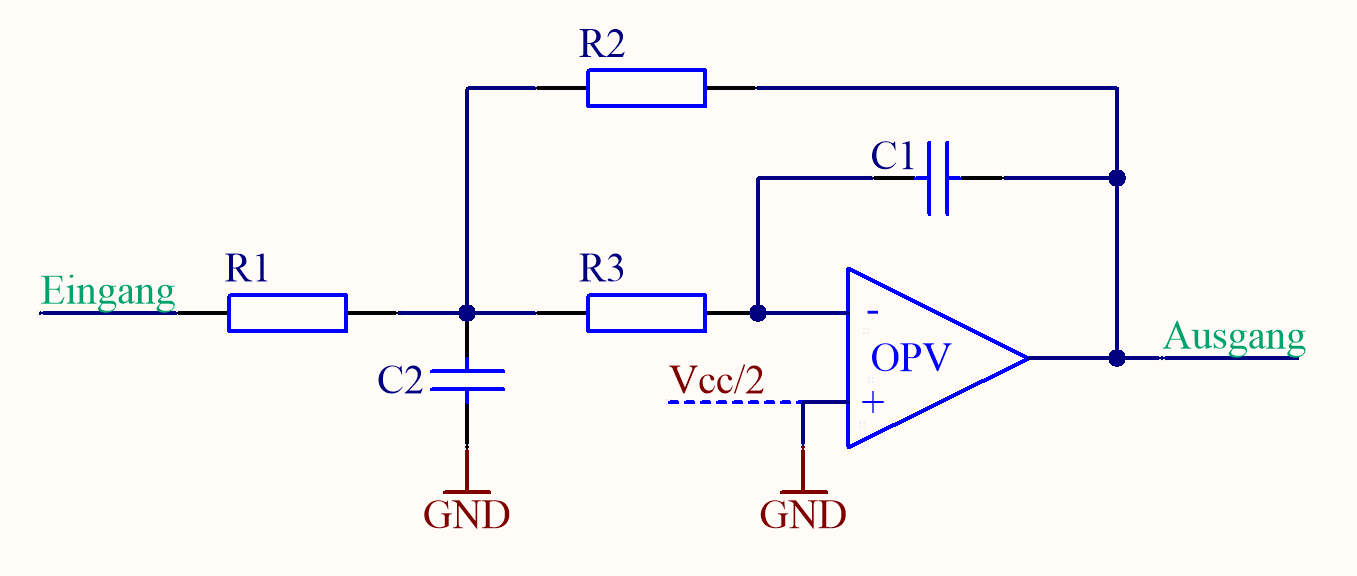
\includegraphics[width=1\textwidth]{img/TPFilterButterworth2Ordnung.PNG}
	\caption{Butterworth-Filter 2. Ordnung}
	\label {fig:abb3.1}
\end{figure}\\

\subsection{Schaltung}
Passend dem Signalverlauf sitzt am Beginn der Schaltung (Abb. \ref{fig:abb3.2}) die erste Regelung über Potentiometer. Anschließend kommt man zu der Addier-Schaltung (Abb. \ref{fig:abb3.3}) welche das Stereo-Signal in ein Mono-Signal wandelt und dadurch Stereo-Effekte wie zB. Balance am \enquote{Mono-Bass} entfernt.\\
Wichtig ist bereits hier die Versorgung der Schaltung. Bedingt durch eine asymmetrische Spannungsversorgung (0...12V) muss am OPV ein Arbeitspunkt eingestellt werden. Dabei handelt es sich um ein absichtliches Anheben des Signals in Y-Richtung bei einem Spannungs-Zeit-Verlauf, sodass die untere Halbwelle des Signals nicht verloren geht. Dafür muss am Plus-Eingang des OPVs der Addier-Grundschaltung und der Butterworth-Filter-Schaltung die halbe Versorgungsspannung angelegt werden, um das beste Ergebnis zu erzielen. Dafür wird an den beiden Plus-Eingängen der OPVs über eine Spannungsteiler-Schaltung aus zwei Widerständen das benötigte $\frac{Vcc}{2}$ angelegt.\\
Um Störungen im OPV zu vermeiden wird sehr nahe an diesem ein 10µF ELKO in der Versorgungsspannungsleitung vorgesehen.\\
Nach Addieren des Stereo-Signals zu einem Mono-Signal kommt dieses zum Aktiven-Tiefpass-Filter(Abb. \ref{fig:abb3.4}). Bevor das gefilterte Signal weiter zum Verstärker geht wird nochmals die Möglichkeit geboten um die Amplitude des Signals anzupassen.
\begin{figure} [h]
	\centering
	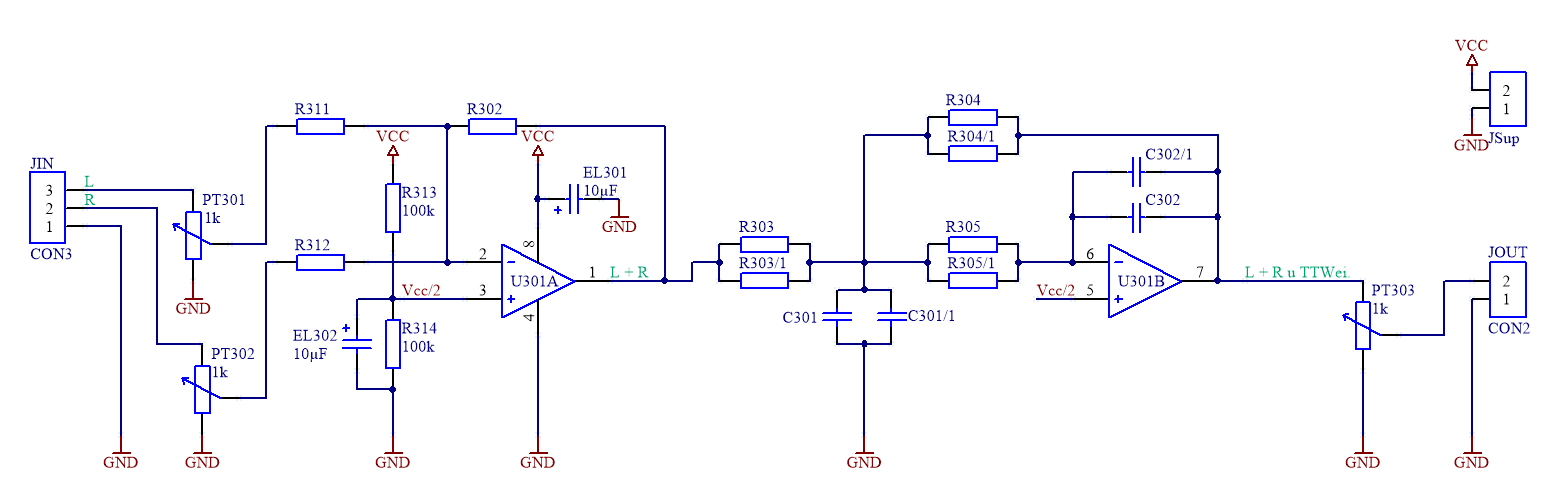
\includegraphics[width=0.8\textwidth]{img/3mTTWeicheruAddiererDiplSchematic.PNG}
	\caption{Schematic Mono-Bass-Addier-Schaltung und Mono-Bass-Weiche}
	\label {fig:abb3.2}
\end{figure}
\begin{figure} [h]
	\centering
%	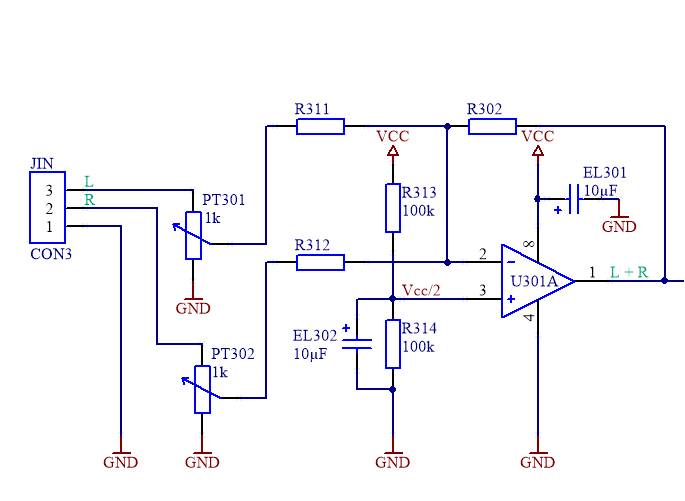
\includegraphics[width=0.8\textwidth]{img/3mTTWeicheruAddiererDiplSchematicTeil1.png}
	\caption{Schematic Mono-Bass-Addier-Schaltung}
	\label {fig:abb3.3}
\end{figure}
\begin{figure} [h]
	\centering
%	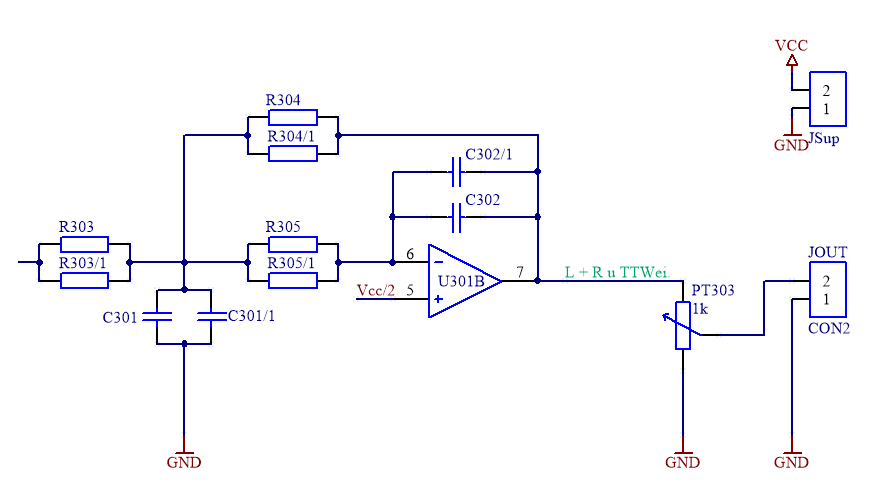
\includegraphics[width=0.8\textwidth]{img/3mTTWeicheruAddiererDiplSchematicTeil2.png}
	\caption{Schematic Mono-Bass-Weiche}
	\label {fig:abb3.4}
\end{figure}



\subsection{PCB}
An einer der vier Seiten der Leiterplatte(Abb. \ref{fig:abb3.5}) wurden alle wesentlichen Ein- und Ausgänge platziert. Eine dreipolige Eingangsstiftleiste für Rechts, Links und Masse. Eine zweipolige Ausgangsstiftleiste für Signal und Masse. Des weiteren darf die Spannungsversorgung nicht fehlen. Wegen größeren Spannungen wurden massivere Stecker verwendet. In diesem Fall handelt es sich um Pol-Klemmen. Zum testen wurde ein zusätzlicher Masse-Printstift angebracht um bei Messungen mit einem Oszilloskop einem besseren Massebezugpunkt zu haben.\\
Die Bauteile wurden nach Möglichkeit gestaffelt, beziehungsweise gruppiert auf der Leiterplatte platziert um den Platzbedarf zu minimieren.
\begin{figure} [h]
	\centering
	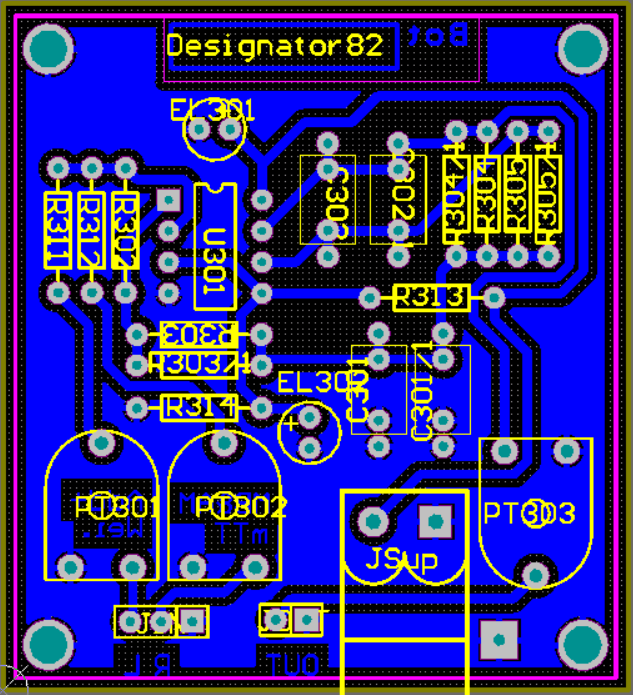
\includegraphics[width=0.8\textwidth]{img/3mTTWeicheruAddierer-PCB.PNG}
	\caption{PCB}
	\label {fig:abb3.5}
\end{figure}


\begin{comment}
%% Altium und Einstellungserklärung + Wichtige Layout-Faktoren
%Beim designen des Leiterplattenlayouts wurden die allgemeinen Altium-Einstellungen vorgenommen und auf die zu berücksichtigenden Layoutpunkte geachtet.
Beim \enquote{Layouten} der Schaltung mussten einige wichtige Faktoren berücksichtigt werden.\\
Wie da wären:\\
\begin{itemize}
	\item EMV-Technische-Faktoren, wie kurze Leiterbahnen
	\item Ausnützen der Printfläche
	\item Mehrfach-Footprints ermöglichen für verschiedene Bauteile
	\item Mechanische Aufhängebohrungen vorsehen
	\item Massefläche bei Möglichkeit vorsehen
\end{itemize}
Leiterplattenspezifische Einstellungen wurden aus den Kriterien der schuleigenen Leiterplattenfertigung übernommen. Zu diesen Einstellungen zählen:\\
\begin{itemize}
	\item Leiterbahnbreite
	\item Leiterbahnabstände untereinander
	\item Restring bei Bohrungen
	\item 
\end{itemize}

\subsection{Inbetriebnahme}
Bereits mit einer simplen Beschaltung kann das Modul in Betrieb genommen werden:
\begin{figure} [h]
	\centering
	\caption{Prinzipschaltung XS3868}
	\label {fig:abb2.3}
%%	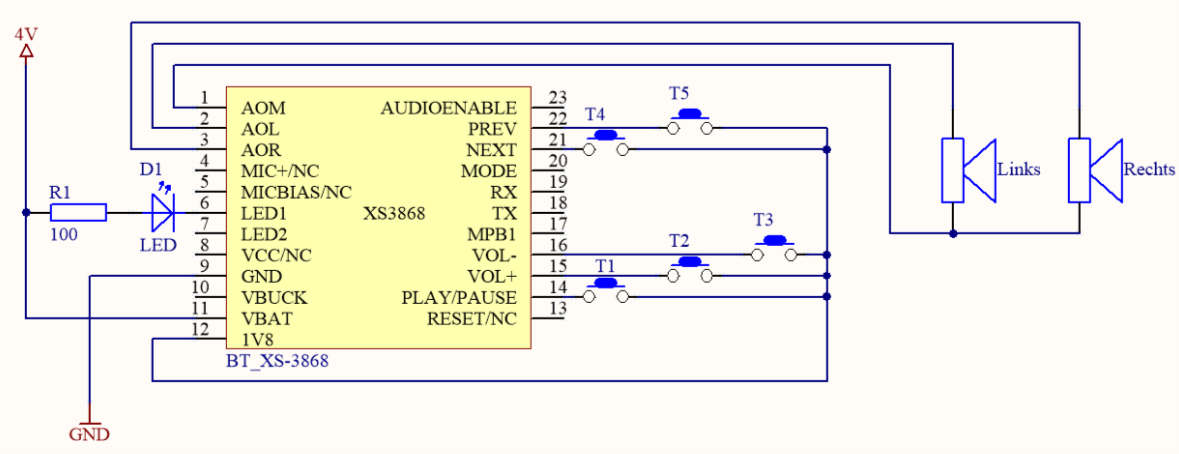
\includegraphics[width=1\textwidth]{schaltungen/XS3868_Prinzipschaltung.png}
\end{figure} \\
Mit dieser Schaltung (Abb. \ref {fig:abb2.3}) kann das Modul bereits ordnungsgemäß arbeiten.\\
Die Versorgungsspannung ist mit 4V etwas höher gewählt damit es nicht zu Ausfällen durch Spannungsschwankungen kommt. Das XS3868-Modul hat eine Stromaufnahme von ca. 30mA beim Starten, 10mA im Stand-By und bis zu 100mA wenn Musik abgespielt wird.\\ \\
Die Status-LED ist, wie in Abbildung \ref {fig:abb2.3} dargestellt, \enquote{Low-Aktiv}. Beim Starten des Moduls und während der Suche nach Geräten blinkt sie durchgehend, wobei sie bei einer bestehenden Verbindung nur die Hälfte der Zeit blinkt.\\ \\
Mit einfachem Betätigen eines Tasters wird die entsprechende Funktion vom Modul ausgeführt, jeweils mit einem Bestätigungston begleitet. Dieser Ton wird auch beim Starten des Moduls abgespielt.\\ \\
Statt die Lautsprecher direkt an das Modul anzuschließen, sollte allerdings noch ein Verstärker verbaut werden.
\newpage


\subsection{Verbindung mit dem Modul}
Wenn der OVC3860 eingeschaltet ist, sucht er andauernd nach BT-Geräten. Mit einem Smartphone findet man das Gerät und kann sich mit einem Standard-PIN-Code (\enquote{0000}) verbinden. Wenn bereits Lautsprecher angeschlossen sind, wird ein Ton abgespielt, der die Verbindung bestätigt. Außerdem hat die Status-LED nun ein anderes Blinkverhalten (Mehrmaliges Blinken mit längeren Pausen).\\ \\
Jetzt ist das Modul bereit Musik abzuspielen. Diese kann vom Smartphone oder vom Modul aus gesteuert werden. Die notwendigen Taster müssen allerdings schon in der Schaltung verbaut sein um die Bedienung der Musik zu ermöglichen.


\subsection{Zusatz-Leiterplatten}
\subsubsection{Allgemeines}
Als Entwicklungsprogramm für beide Leiterplatten wurde  \enquote{Altium Designer 13.3} verwendet. Die Schaltung wurde in diesem Programm gezeichnet, das Layout für die Leiterplatten angefertigt und entflechtet. Es wurden einseitige Platinen verwendet, da doppelseitige nicht notwendig waren.


\subsubsection{Adapter-Board}
Da das Modul in SMD-Bauform gefertigt ist, wurde ein Adapter-Board (Abb. \ref{fig:abb3.1}) vorgesehen um eine einfachere Handhabung mit dem Modul zu ermöglichen. Als Anschlussmöglichkeiten werden Stiftleisten verwendet.\\
Die Schaltung ist deshalb auch sehr simpel aufgebaut:
\begin{figure} [h]
	\centering
	\caption{Schaltung des Adapter-Boards}
	%%\label {fig:abb3.1}
%%	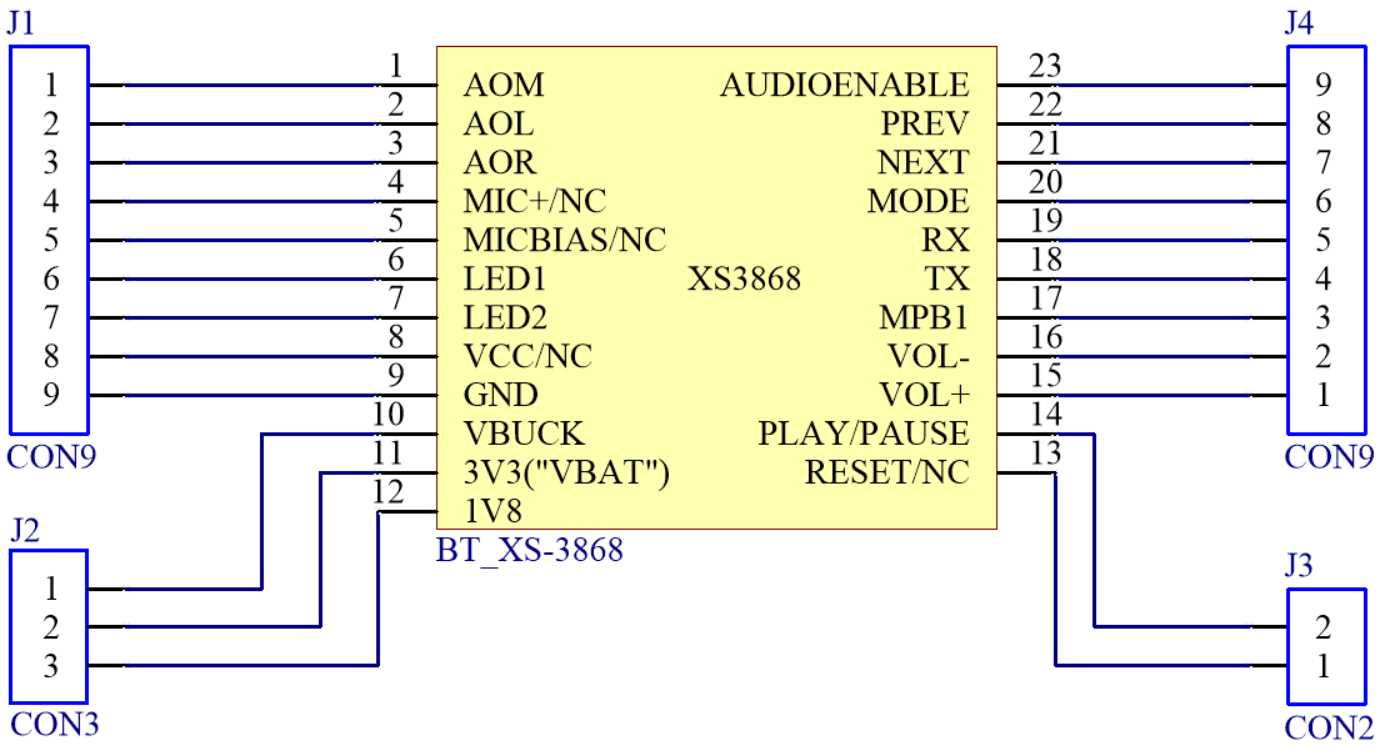
\includegraphics[width=1\textwidth]{schaltungen/adapter_sch.png}
\end{figure} \\
Jeder Pin bekommt auch auf dem Adapter einen eigenen Pin auf der Stiftleiste.
\newpage
Das PCB (Abb. \ref{fig:abb3.2}) ist, wie bereits erwähnt, einseitig aufgebaut:
\begin{figure} [h]
	\centering
	\caption{PCB des Adapter-Boards}
%%	\label {fig:abb3.2}
%%	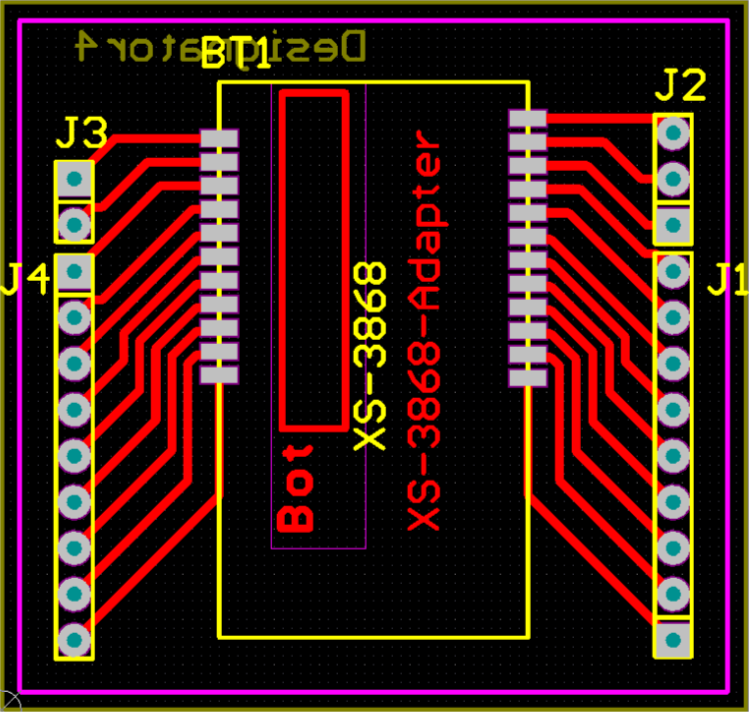
\includegraphics[width=1\textwidth]{schaltungen/adapter_pcb.png}
\end{figure} \\
Mit diesem PCB kann da BT-Modul nun besser getestet und auch weiterverwendet werden. Gemeinsam mit diesem Adapter kommt es auch auf das Hauptboard.
\newpage


\subsubsection{Hauptboard}
\minisec{Funktion}
Das Hauptboard wird hauptsächlich zur Versorgung des BT-Moduls, aber auch zur Weiterverarbeitung des Audio-Signals verwendet. Darüber hinaus ist eine Additionsschaltung vorgesehen, die das Signal des BT-Moduls mit einem zweiten, von einem Klinken-Eingang zugeführten, Signal vermischt. Die Lautstärke von diesem zweiten Audio-Signal kann über ein Stereo-Potentiometer geregelt werden. \\
Weiterhin sind die Pins zur Bedienung der Musik an einen 2x5-Wannenstecker herausgeführt. Zugang zur seriellen Schnittstelle wird auch ermöglicht.

\minisec{Schaltung}
Die Schaltung (Abb. \ref{fig:abb3.3}) des Hauptboards ist in mehrere Teile aufgeteilt und wird deshalb auch einzeln erklärt.
\begin{figure} [h]
	\centering
	\caption{Schaltung des Hauptboards (Versorgung + BT-Modul)}
%%	\label {fig:abb3.3}
%%	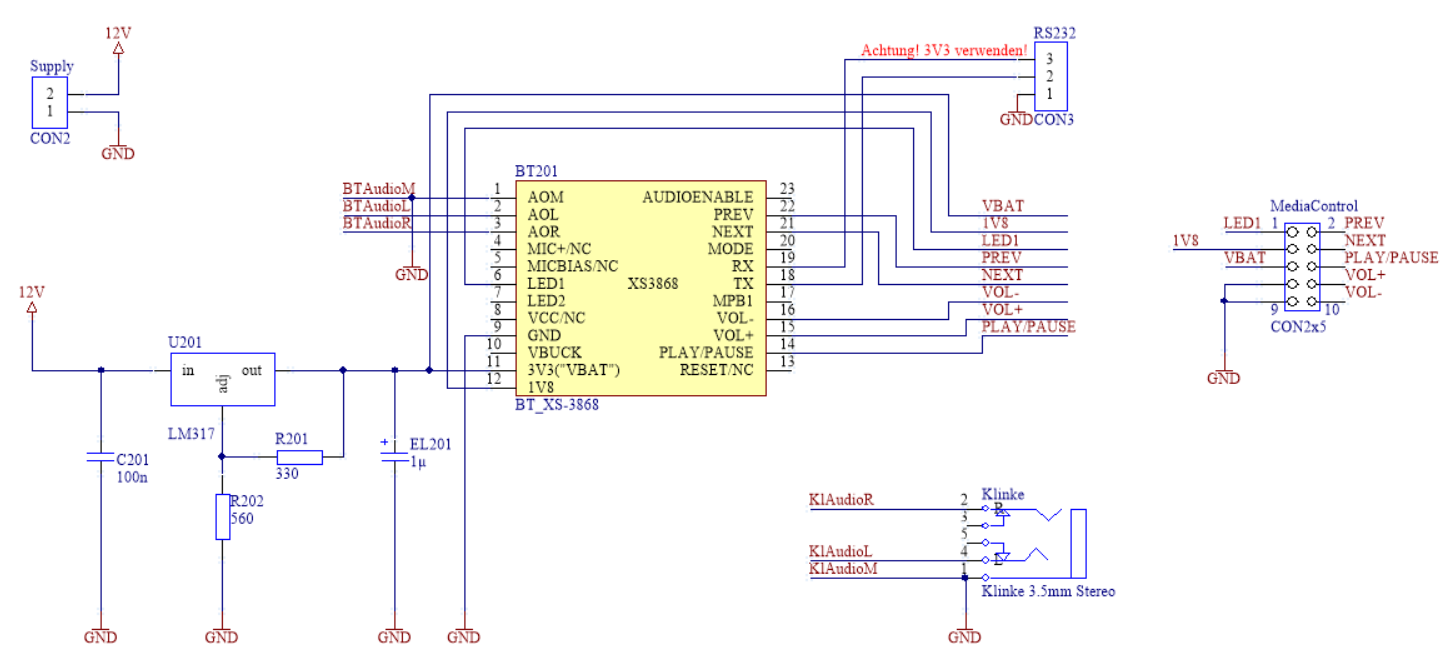
\includegraphics[width=1\textwidth]{schaltungen/hauptboard_sch1.png}
\end{figure} \\
In diesem Teil der Schaltung ist zu sehen: die Versorgungsbuchse, die Versorgungsschaltung für das BT-Modul, das BT-Modul mit herausgeführten Pins und die Klinken-Buchse.\\
Der Spannungsregler LM317 (Bezeichnung: U201) stellt eine Versorgungsspannung von 3,9V für das BT-Modul ein. Mit einer maximalen Stromaufnahme von 100mA ergibt sich folgende Verlustleistung:
\begin{equation}
	P_{max} = 7,9V * 100mA = 0,79W
\end{equation}
Deshalb wird auch kein Kühlkörper benötigt, es wird aber trotzdem eine Alu-Platte an den LM317 geschraubt um sicher zu gehen. \\
Ein eigener Stecker (Stiftleiste) für die Versorgung (12V) sowie die UART-Schnittstelle (RS232) sind auch vorgesehen. Der Wannenstecker (hier: \enquote{MediaControl}) ist mit allen wichtigen Pins des Moduls verbunden und verbindet eine Frontplatine mit dem Hauptboard. \\ \\
Die Klinkenbuchse wird in der folgenden Additionsschaltung(Abb. \ref {fig:abb3.4}) weiterverwendet:
\begin{figure} [h]
	\centering
	\caption{Schaltung des Hauptboards (Additionsschaltung)}
%%	\label {fig:abb3.4}
%%	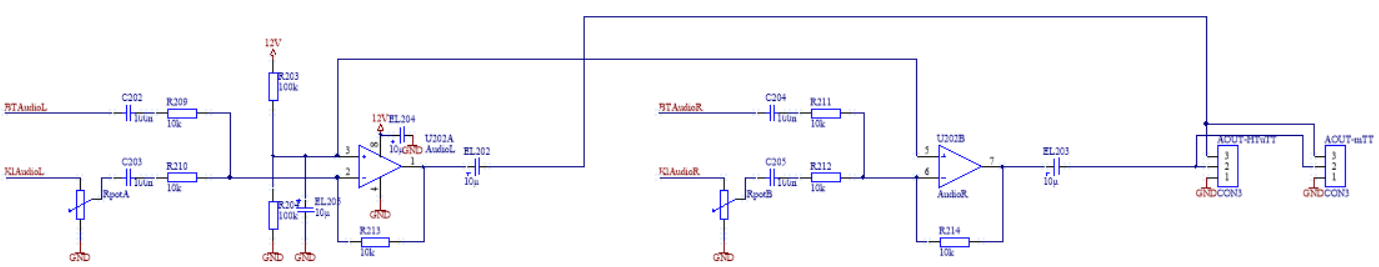
\includegraphics[width=1\textwidth]{schaltungen/hauptboard_sch2.png}
\end{figure} \\
Vergrößert:
\begin{figure} [h]
	\centering
	\caption{Schaltung des Hauptboards (linker Teil der Additionsschaltung)}
%%	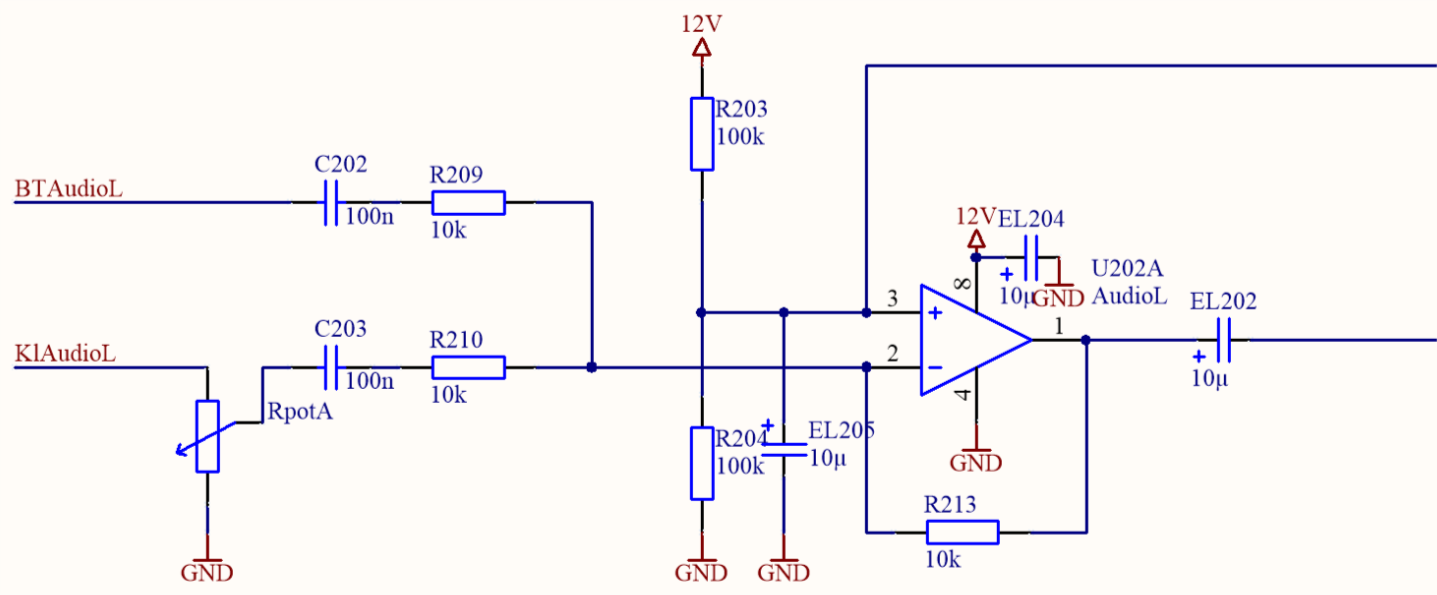
\includegraphics[width=1\textwidth]{schaltungen/hauptboard_sch2_zoom.png}
\end{figure} \\
Mithilfe dieser OPV-Schaltung werden die zwei Audio-Signale (ein Addierer pro Kanal) addiert. Das Signal vom Klinkeneingang kann zuvor noch mit einem Potentiometer abgeschwächt werden.\\
Der Arbeitspunkt bei 6V am Pin 3 wird benötigt um am Ausgang eine Spannung von $\pm$6V zu erreichen. Der OPV wird hier als invertierender Verstärker mit Verstärkung 1 aufgebaut, aber er addiert hier die zwei Signale zusammen auf ein Ausgangssignal.

\minisec{PCB}
Die Platine(Abb. \ref {fig:abb3.6}) für das Hauptboard sollte möglichst kompakt sein und alle Eingänge oder Bedienelemente auf einer Seite (hier rechts) haben. Das BT-Modul wird samt Adapter auf zwei Stiftleisten gesteckt. Darunter werden keine Bauteile verwendet, weil es sonst zu eng wäre. Des weiteren wären Bauteile unter dem Adapterprint während der Testphase unvorteilhaft, da diese schwerer zugänglich sind.
\begin{figure} [h]
	\centering
	\caption{PCB des Hauptboards}
%%	\label {fig:abb3.6}
	%%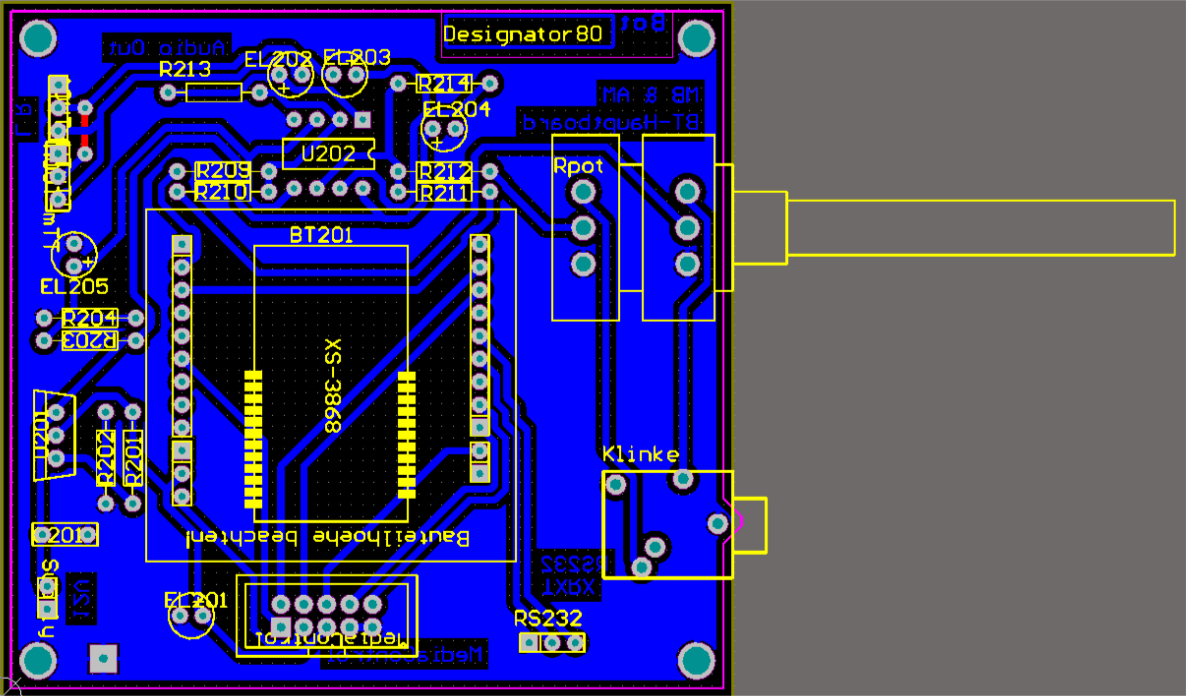
\includegraphics[width=1\textwidth]{schaltungen/hauptboard_pcb.png}
\end{figure}
\newpage


\subsubsection{Frontplatine}
\minisec{Funktion}
Diese Platine ist eigentlich eine Erweiterung des Hauptboards. Es wird mit dem Hauptboard über einen 2x5-Wannenstecker verbunden und auch versorgt. Sonst sind nur die Taster zur Bedienung des BT-Moduls, sowie die Status-LED verbaut.

\minisec{Schaltung}
Die Taster werden jeweils mithilfe eines Kondensators entprellt. Die Höhe der Taster reicht über die Kondensatoren hinaus um eine Bedienung zu ermöglichen. (Abb. \ref{fig:abb3.7})
\begin{figure} [h]
	\centering
	\caption{Schaltung der Frontplatine}
%%	\label {fig:abb3.7}
	%%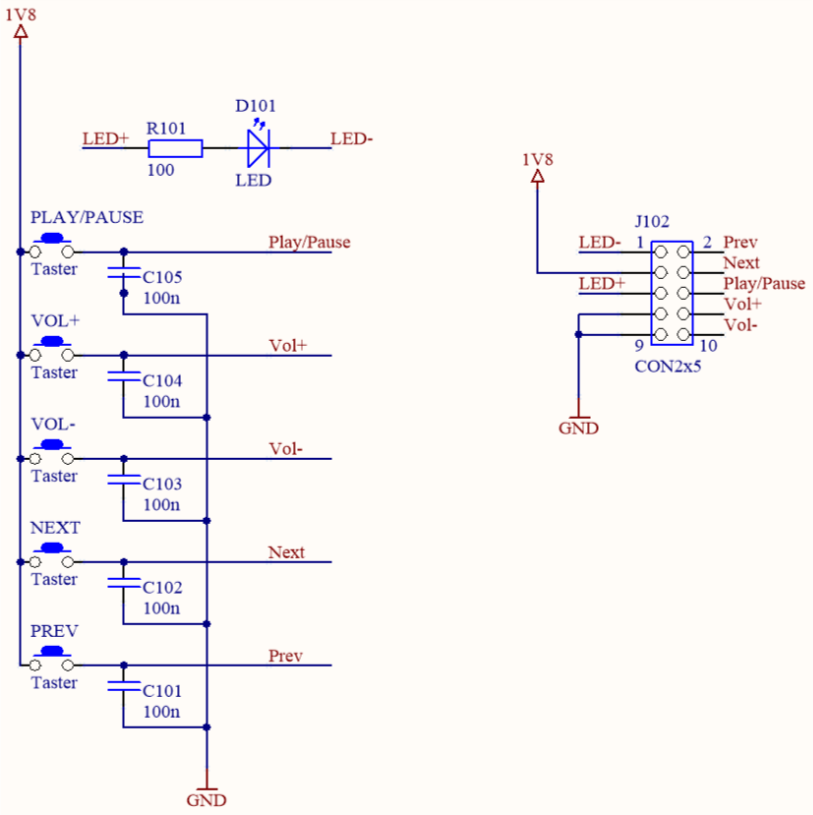
\includegraphics[width=0.7\textwidth]{schaltungen/front_sch.png}
\end{figure} \\
Jeder der Taster ist mit dem 1,8V-Pin des Moduls verbunden und geht dann weiter auf den entsprechenden Funktionspin. Die Bezeichnung \enquote{LED+} entspricht der Versorgungsspannung (\enquote{VBAT} = 3,9V) des Moduls. \enquote{LED-} ist mit dem Ansteuerungssignal am BT-Modul verbunden (Pin 6).

\minisec{PCB}
Das PCB (Abb. \ref {fig:abb3.8}) der Frontplatine soll ebenfalls so klein wie möglich aber von der Bedienung her sinnvoll aufgebaut sein.
\begin{figure} [h]
	\centering
	\caption{PCB der Frontplatine}
%%	\label {fig:abb3.8}
	%%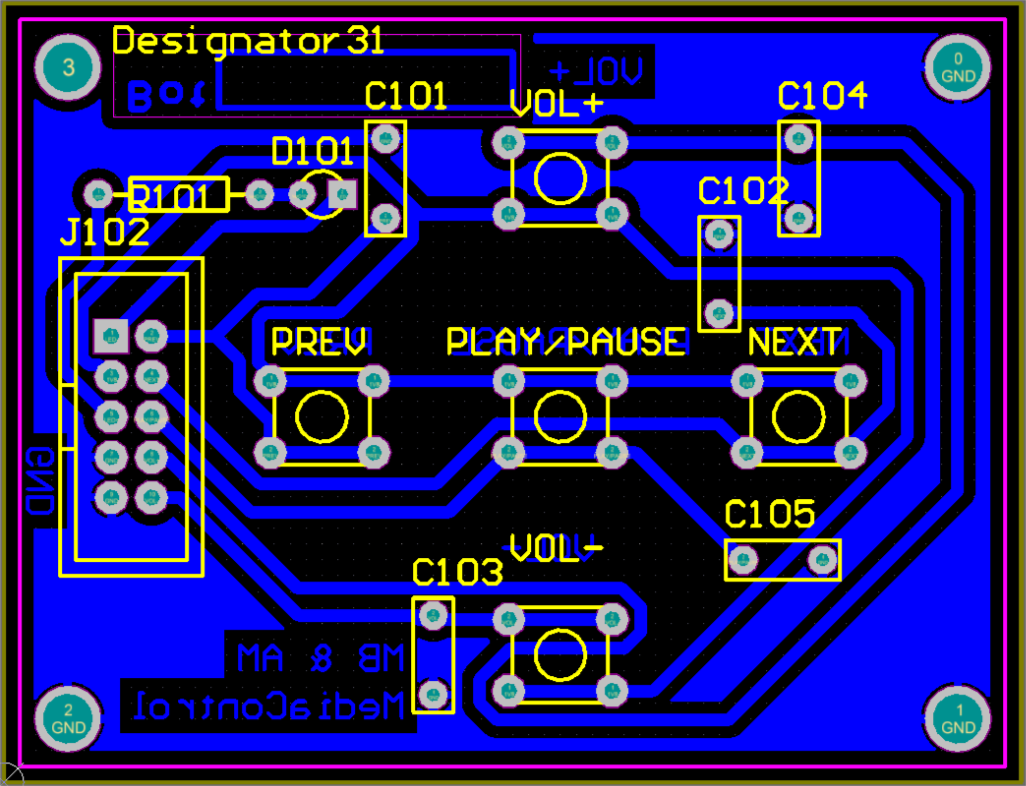
\includegraphics[width=1\textwidth]{schaltungen/front_pcb.png}
\end{figure} \\
Die Taster wurden in einem Kreuz aufgebaut, wobei an der linken oberen Ecke die Status-LED verbaut wurde.
\end{comment}






